\documentclass{article}
\usepackage[utf8]{inputenc}
\usepackage[a4paper, total={6in, 8.5in}]{geometry}
\usepackage{indentfirst}
\usepackage{listings}
\usepackage{fancyvrb}
\usepackage{array}
\usepackage{graphicx}
\usepackage{float}
\usepackage{xcolor}

\definecolor{codegreen}{rgb}{0,0.6,0}
\definecolor{codegray}{rgb}{0.5,0.5,0.5}
\definecolor{codepurple}{rgb}{0.58,0,0.82}
\definecolor{backcolour}{rgb}{0.95,0.95,0.92}

\lstdefinestyle{mystyle}{
    backgroundcolor=\color{backcolour},   
    commentstyle=\color{codegreen},
    keywordstyle=\color{magenta},
    numberstyle=\tiny\color{codegray},
    stringstyle=\color{codepurple},
    basicstyle=\ttfamily\footnotesize,
    breakatwhitespace=false,         
    breaklines=true,                 
    captionpos=b,                    
    keepspaces=true,                 
    numbers=left,                    
    numbersep=5pt,                  
    showspaces=false,                
    showstringspaces=false,
    showtabs=false,                  
    tabsize=2
}

\lstset{style=mystyle}

\usepackage{caption}
\usepackage{subcaption}

\title{Advanced programming for HPC Labwork 2- Report}
\author{Nguyen Quoc Thong - M21.ICT.010}
\date{December 2022}

\begin{document}

\maketitle

\section{Project}
The project goal is to compare the computation time of the CPU and GPU by converting an image from RGB to grayscale and finding the optimal block size value. the project environment is CPU: Intel Core i7-7720HQ and GPU: NVIDIA GEFORCE GTX 1050

\section{Implementation}
The labwork can be concluded in the following step:
\begin{itemize}
    \item Load an RGB image into a 3-Dim array
    \item Convert RGB image into a grayscale image
    \item Compare the time taken to compute from RGB to grayscale with CPU and GPU
\end{itemize}

The following pictures are the base RGB image and the grayscale images converted with CPU and GPU respectively. The image shape are (634, 640, 3)

\begin{figure}[H]
    \center{
        
\includegraphics[scale=0.5]{lechonk.jpg}
    \caption{Sample image}
    }
\end{figure}

\begin{figure}[H]
    \center{
        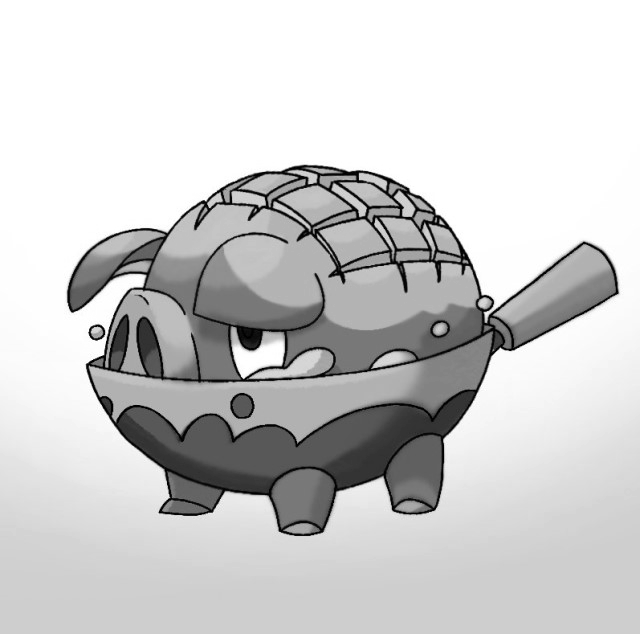
\includegraphics[scale=0.5]{grayed.png}
    \caption{Grayscale image converted with CPU}
    }
\end{figure}
\begin{figure}[H]
    \center{
        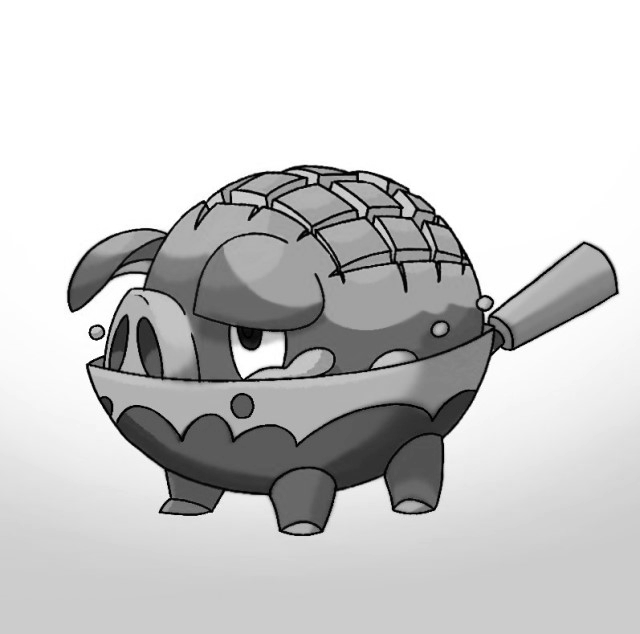
\includegraphics[scale=0.5]{gpu.png}
    \caption{Grayscale image converted with GPU}
    }
\end{figure}

\paragraph{CPU:} The following function is the code to convert the image from RGB to gray with CPU
\begin{lstlisting}[language=Python]
def rgbToGray(img):
    r,g,b =image[:,:,0]*0.2989,image[:,:,1]*0.5870,image[:,:,2]*0.1140
    gray = r+g+b
    return gray
\end{lstlisting}
The processing time is CPU: 0.04515552520751953

\paragraph{GPU:} The following function is the code to convert the image from RGB to gray with CPU. 
\begin{lstlisting}[language=Python]
@cuda.jit
def grayscale(src, dst):
    tidx = cuda.threadIdx.x + cuda.blockIdx.x * cuda.blockDim.x
    g = (src[tidx, 0] + src[tidx, 1] + src[tidx, 2]) / 3
    dst[tidx] = g
\end{lstlisting}
The processing time is GPU: 0.33090710639953613 with a block size of 64


\paragraph{Block sizes:} To find the optimal block size of the GPU, the function above was also tested with different block sizes [16, 32, 64, 128, 256, 512, 1024]. The following figure shows the time compute over different block sizes.

\begin{figure}[H]
    \center{
        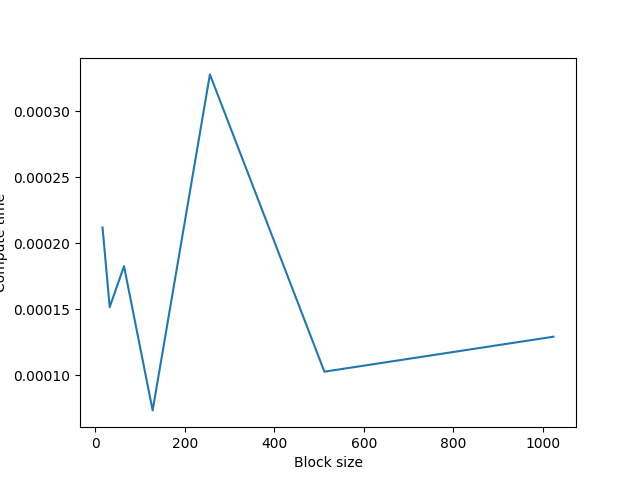
\includegraphics[scale=0.8]{Execution over block size.png}
    \caption{Sample image}
    }
\end{figure}

\textbf{Discussion :} The block size with the fastest computation time is 128 which have much lower computation time again using CPU.

\end{document}